\chapter{Introduction}
\label{chap:Intro}
This chapter presents the fundamentals of our project. This includes the background and purpose of it as well as the people involved.

\section{Project Name}
\label{sec:IntroProjName}
This is a report on the project "Alternative Spaces - the digital prototype", herein referred to as "ASpaces", or "The Digital Prototype". \\
It is part of the larger research project "Alternative Spaces", which explores the possibilities of creating alternative city spaces in cooperation with urban youth, artists, architects, journalists and scientists. It is currently planning to run a test project in Tøyen in Oslo.

\section{Project Description}
\label{sec:IntroProjectDescr}
This project is part of the course TDT4290: Customer Driven Project at NTNU. The purpose of the course is to give students experience working on IT projects, by making the projects as close to a real working situation as possible. Steps involved in the project includes, but are not limited to, planning and management, software development, customer relations, and group dynamics. \\
This group was given the task of developing a platform to facilitate "digital sharing of [visual, physical and mediated expressions] for youth." The aim is mainly to give ideas of how such a platform could work, and to create a prototype capable of demonstrating what a complete system would be capable of. \\
The description of the project from AFI is as follows:

\textit{"With the increasing commercialization of city spaces, youth citizens have less room to express themselves, whether it is through visual, physical or mediated expressions like movement, dance, street art, sports activities or media outlets. The research project “Alternative Spaces” will explore the possibilities of creating alternative city spaces (both material and virtual) together with groups of youth, dancers, artists, landscape architects, journalists and scientists. Visual expression, digital media and film will make up both the methodological and empirical part of the project. \\
This assignment is to design a new platform experience that can facilitate digital sharing of such expressions across urban communities globally. As many of the project activities will be happening “on the ground” there is an acute need for a commercial-free digital hub where youth can upload, share and create content that strengthens their local engagement, expression of ideas and experimental thinking when it comes to participation and political influence on the development of their city spaces. \\
The project is in the early phase of development, where idea generation and the creating of connections and network of researchers and practitioners are integral. There will thus be plenty of opportunities for the students to influence the overall project design. During the fall of 2014 the project will arrange a workshop where all relevant actors will be invited to work together on related issues. This will be a venue for the students in the “customer driven project” to engage directly with the potential users of their platform. The case study of the first phase of the project will be Oslo, but Trondheim may be included as a complementary case if the student group finds the project attractive. 
The project assignment will consist of the following activities:
\begin{itemize}
\item Produce a user-oriented case, in dialogue with the research group
\item Participate and present pilot idea in “Alternative Spaces” workshop
\item Produce design suggestions, map needs and find the relevant technology for the pilot
\item Develop the web interface for analysis and representation
\item Evaluate design and technical solution and recommend further development"
\end{itemize}}

We decided to create a web application focused on the idea of connecting urban youth sharing similar interests or hobbies by planning open events and sharing media at different locations. It allows you to search for media and events on a map based on these interests, and will show the most relevant matches. To more easily facilitate the uploading of pictures, we have also created an accompanying Android application for this purpose. This app currently only has the functionality of sharing media, to better illustrate how users would interact with the system for the customer. A thorough description of ideas for further development can be found in chapter INSERT REFERENCE HERE (EXAMPLE IN COMMENT) %\ref{chap:FurtherWork}.


\section{Customer}
\label{sec:IntroCustomer}

Our customer is the Work Research Institute (AFI), represented by the researchers in charge of the "Alternative Spaces" project, Aina Landsverk Hagen and Arne Bygdås. \\
The main goals of the institute is to produce research based knowledge on organization, leadership, and the work environment. Of particular interest are organizational and leadership structures that strengthen conditions for learning, business development, involvement and restructuring in both the public and private sector.

\begin{figure}[ht!]
\centering

\includegraphics[width=\linewidth]{./Introduction/img/afi}
\caption{The Work Research Institute \label{fig:IntroAfi}}
\end{figure}

\section{Stakeholders}
\label{sec:IntroStakeholders}

The stakeholders of this project are the people directly or indirectly involved in the development or results of the project. The stakeholders have an interest in the project and are either affected by or affect the development process or the end results. Four stakeholders of the Alternative Spaces project have been identified.

\subsection{Project Team}
\label{subsec:IntroStakeProjectTeam}

The project team is composed of seven students from the Norwegian University of Technology (NTNU). All members of the team are on their Master's degree either in Informatics or Computer Science Engineering. It's an international team with five students native to the University and two exchange students, one from India and one from Germany. The diversity adds cultural flavor and variety of viewpoint. The project team, counselled by the advisor, is mainly focused on satisfying the customer by delivering a fully functional prototype of the product within the given timeframe. To achieve this the team works with the system development, testing, and documentation of the Alternative Spaces project.

\begin{minipage}{\linewidth}
\centering
%\setlength{\tabcolsep}{22pt}
\textbf{Team:} \\
\smallskip
\rowcolors{1}{blue!20}{blue!10}
\begin{tabular}{ |p{5cm} p{35mm}| }
	\hline
	\cellcolor{gray!25} \begin{tabular}{l} \cellcolor{gray!25} \textbf{Name and E-Mail} \end{tabular} & \cellcolor{gray!25} \textbf{Study} \\
	\hline
	\begin{tabular}{l} Jonas Foyn Therkelsen \\ \texttt{jonasft@stud.ntnu.no} \end{tabular} & Computer Science, Software \\
	\begin{tabular}{l} Brage Ekroll Jahren \\ \texttt{brageej@stud.ntnu.no} \end{tabular} & Computer Science, Artificial Intelligence \\
	\begin{tabular}{l} Valerij Fredriksen \\ \texttt{valerijf@stud.ntnu.no} \end{tabular} & Computer Science, Artificial Intelligence \\
	\begin{tabular}{l} Hans Olav Slotte \\ \texttt{slotte@stud.ntnu.no} \end{tabular} & Computer Science, Artificial Intelligence \\
	\begin{tabular}{l} Yngve S. Bloch-Hoell \\ \texttt{yngvesbl@stud.ntnu.no} \end{tabular} & Computer Science, Artificial Intelligence \\
	\begin{tabular}{l} Julia Schneider \\ \texttt{juliasch@stud.ntnu.no} \end{tabular} & Informatics \\
	\begin{tabular}{l} Manasa Vallamkondu \\ \texttt{manasav@stud.ntnu.no} \end{tabular} & Informatics \\
	\hline
\end{tabular}
\end{minipage}

\subsection{Customer}
\label{subsec:IntroStakeCustomer}
The customer, also specified in the section above, is the Work Research Institute (AFI), represented by the researchers in charge of the Alternative Spaces project, Aina Landsverk Hagen and Arne Bygdås. The customers are concerned with the iterative deliverables from each sprint, evaluating them and giving feedback to the Scrum Team so that the product will meet their expectations.

\begin{minipage}{\linewidth}
\centering
\setlength{\tabcolsep}{22pt}
\textbf{Customer:} \\
\smallskip
\rowcolors{1}{blue!20}{blue!10}
\begin{tabular}{|l l|}
    \hline
    \cellcolor{gray!25} \textbf{Name} & \cellcolor{gray!25} \textbf{E-mail} \\
    \hline
    Aina Landsverk Hagen & \texttt{aina.hagen@afi.hioa.no} \\
    Arne Bygd\aa s & \texttt{arne.bygdas@afi.hioa.no} \\
    \hline
\end{tabular}
\end{minipage}

\subsection{Advisor}
\label{subsec:IntroStakeAdvisor}

The advisor of the group is Gleb Sizov of IDI at NTNU. As the advisor of the Alternative Spaces group, he is concerned with the progression of the group, focusing on group dynamics and the progress of system development and the report. 

\begin{minipage}{\linewidth}
\centering
\setlength{\tabcolsep}{22pt}
\textbf{Advisor:} \\
\smallskip
\rowcolors{1}{blue!20}{blue!10}
\begin{tabular}{|l l|}
    \hline
    \cellcolor{gray!25} \textbf{Name} & \cellcolor{gray!25} \textbf{E-mail} \\
    \hline
    Gleb Sizov & \texttt{glebsv@gmail.com} \\
    \hline
\end{tabular}
\end{minipage}

\subsection{End Users}
\label{subsec:IntroStakeEndUsers}
These stakeholders are the end users of the complete system that will be Alternative Spaces. Currently there are no users, but the targeted audience is youth living in urban regions with high population densities. The end users want to use the site to satisfy social, entertainment and educational needs. Currently only a few external users have tested and evaluated the product and given valuable feedback that directly influenced the design of the prototype.

\section{Project Plan}
\label{sec:IntroProjPlan}

\section{Methodology}
\label{sec:IntroMethod}
During the preliminary studies, two development processes were considered, the waterfall model and the scrum model. As a result of the preliminary studies the scrum model was chosen. This chapter deals with a short justification of why scrum was the best choice, and how we adjusted the process to fit this project.

\subsection*{Scrum, our choice in methodology}
\label{subsec:IntroMethodChoice}
At the beginning of this project, the customer presented their vision, but did not present us with any concrete requirements for the final product. As a result of this, it was important to choose a development process where requirements can be changed and extended easily. For this, scrum was the best fit. Another reason for choosing scrum was the needed involvement of end users for feedback. This also required us to be able to adapt to change, as feedback often leads to changes to the requirements. Being a project with very few initial requirements it was important to involve end users as early as possible, and present a  product iteration as often as possible to the customer. With these two requirements for the project, scrum was the best choice. A detailed description of scrum in comparison with the waterfall model is termed in chapter JULIAC1 %\ref{JULIA_C1}.

\subsection*{Required adjustments}
\label{subsec:IntroMethodAdjust}
Certain aspects of the scrum methodology, as described in chapter JULIAC1, did not fit the project team. Because of this, adjustments to the method had to be made. Due to other courses and assignments, it was not feasible for the team to meet every day, and we had to reduce the daily stand up meetings to biweekly meetings. Team members were responsible for reporting their work status to the scrum master. That way the work progress could be tracked outside of meetings. Our scrum team created a product backlog and at the start of each sprint selected which of the requirements should be fulfilled by the end of that sprint.

%TODO CHECK PHRASING
\paragraph{} In contrast to traditional scrum, we had sprints with the duration of only one week in the beginning of the project. That way it was easier to manage the sprint, when no team members had prior experience working with scrum. After the first few weeks the sprint duration was extended to approximately two weeks. 

%TODO CHECK PHRASING
\paragraph{} At the end of each sprint we had a sprint delivery where we presented the product to the customer. This made it possible for the customer to see the progress of the project, and their frequent feedback gave us the ability to ensure that the project was headed in the right direction by finding problems early. The retrospective meeting after each sprint was helpful to get an overview over potential problems during the last sprint and what we could do to improve the work process for the next sprint. 

%TODO CHECK PHRASING
\paragraph{} The project work was divided into two groups. The first group would focus on implementation and the second group on the report. To track which people were working on what tasks, we used the Issue Tracker Tool YouTrack. This tool helped us assign tasks to team members and set the status of tasks. All team members could see what the others were working on and when they were finished. It also gave us an integrated burndown chart, which shows the work left versus the time left.


\section{Group Organization and Project Management}
\label{sec:IntroGroupOrg}
Our group consists of seven people, and most of them have more than one role within the team. There are three main roles in a scrum team; product owner, scrum master and scrum team. The overall structure of this group is flat, since the group is fairly small.

\subsection{Roles}
\label{subsec:IntroGroupOrgRoles}
\paragraph{The Project Lead/Scrum Master} is responsible for the overall progress of the project and organizational tasks such as planning and workload. The project lead has to make plans for sprints, meetings and deliveries and maintain contact with the customer and supervisor.

\paragraph{Team}
\begin{itemize}
    \item \textbf{The Implementation Lead} has  final responsibility over the system. He is responsible for keeping track of what needs to be done on the system to make it ready for delivery. He also has a responsibility to be available to help other with any problems they might have regarding the implementation.
    \item \textbf{The Requirements Specialist's} initial responsibility is making sure a system requirements document is created and important use cases are ready. They also have a responsibility to make sure the final system fulfills these requirements.
    \item \textbf{The Document Managers} are responsible for the work done on the report. They are responsible for assigning sections that need to be written in the document and making sure the different parts match each other.
    \item \textbf{The Test Managers} work closely with the requirements specialist to make tests for the final system test, as well as doing tests while development is ongoing. They are responsible for making a test plan and making sure the plan is executed in the final stages of the project.
    \item \textbf{Developers} are responsible for creating quality code for any task they may be assigned to, and keeping the repository up to date with their code. They also have to make sure to keep the time spent up to date on our backlog, and to take responsibility for any open issues they are able to solve.
    \item \textbf{Architects and designers} are responsible for the overarching design and higher level system architecture. As with developers, they have to make sure to keep their time tracking up to date, and to be ready to take care of any issues.
\end{itemize}

\subsection{Allocation of Roles}
\label{subsec:IntroGroupOrgAllocation}
Each member of our team has at least one role with its accompanying responsibilities. We selected these based on the needs of the project and the wishes of the group. In addition to any roles allocated here, all group members are expected to be able to jump in and do a critical task as needed, and the Project Lead is responsible for keeping track and allocating these tasks. We tried to limit the number of roles, since the group is fairly small.

\begin{minipage}{\linewidth}
\centering
%\setlength{\tabcolsep}{22pt}
\rowcolors{1}{blue!20}{blue!10}
\begin{tabular}{|l l|}
    \hline
    \textbf{Project Lead} & \begin{tabular}{l}
                            Jonas F. Therkelsen \\
\end{tabular} \\
    \textbf{Implementation Lead} & \begin{tabular}{l}
                                   Valerij Fredriksen \\
\end{tabular} \\
    \textbf{Requirements Specialists} & \begin{tabular}{l}
                                        Brage E. Jahren \\
\end{tabular} \\
    \textbf{Developers} & \begin{tabular}{l}
                 Yngve Bloch-Hoell \\
                 Valerij Fredriksen \\
                 Brage E. Jahren \\
                 Hans Olav Slotte \\
                 Manasa Vallamkondu \\
    \end{tabular} \\
    \textbf{Document Manager} & \begin{tabular}{l}
                                Julia Schneider \\
    \end{tabular} \\
    \textbf{Architects and Designers} & \begin{tabular}{l}
                               Brage E. Jahren \\
                               Valerij Fredriksen \\
                               Jonas F. Therkelsen \\
    
    \end{tabular} \\
    \hline
\end{tabular}
\end{minipage}

%TODO ONE PASS DONE RECHECK
\section{Project Phases}
\label{sec:IntroProjPhases}
The team divided the project into seven different phases. these consist of the preliminary studies, five sprints and a final phase with documentation and delivery. The preliminary studies includes brainstorming and development of the idea, rough designs and mockups made in dialog with the customers. Following the preliminary studies were the sprints. Each sprint was between one and two weeks long, focusing on implementing the system, group dynamics, and contact with the supervisor and customers. The final phase of the project consists of documentation and delivery of the report and product. No new features to be developed during this phase, but the system is tested to be fully functional and ready for delivery. 

\subsection{Preliminary Studies}
\label{subsec:IntroProjPhasesPrelim}
The preliminary studies took place during the first two weeks of the project. At our initial meeting with the customers, the project team was presented with the customer’s vision of a digital product. Over the next two weeks, the team met on almost a daily basis developing the concept for a product based on the vision presented by the customer. When the concept was approved, different roles were assigned to the members of the group, and technlogy platforms and frameworks decided upon and basic implementation started. We also made some initial assessments of the different development methodologies during this phase, but no final conclusion was made about whether to choose scrum or the waterfall method.

\subsection{Sprints}
\label{subsec:IntroProjPhasesSprints}
The Sprints of the project comprise the next eight weeks of the project. There were six separate sprints, of which a couple were two week long sprints. The main focus of the sprints was the system development and creating first drafts of the relevant sections of the report. Each sprint has it’s own corresponding chapter in the report,ref{chap:Sprint1} through ref{chap:Sprint5}, where the efforts of each sprint are described in depth.

\subsection{Documentation and Delivery}
\label{subsec:IntroProjPhasesDocDel}
%TODO

\section{Risk Management}
\label{sec:IntroRiskMan}
We will now focus on the risk management of the project. The whole project will be analysed and risks are grouped by the following criteria:
\begin{itemize}
\item \textbf{A} Group communication
\item \textbf{B} Issues with the customer
\item \textbf{C} Risks in relation to planning
\end{itemize}
%TODO CHECK PHRASING
Once each risk has been placed into a category, the first letter of its ID has been determined. All risks in a category are then numbered to give them their final ID. Once risks have been decided, we moved on to deciding their probabilities and consequences in order to evaluate how problematic they would be for the project. The following table shows the meaning of each of the consequence levels.

\begin{minipage}{\linewidth}
\setlength{\tabcolsep}{10pt}
\centering
\rowcolors{1}{blue!20}{blue!10}
\begin{tabular}{ |l|p{5cm}| }
	\hline
	\multicolumn{2}{|c|}{\cellcolor{gray!25} Consequence Levels} \\
	\hline
	High & This risk is a major problem. It has a big impact on the project, especially on finishing the project in the given time.\\
	Medium & This risk is big, but still manageable. Mostly this leads to more work for the team members. \\
	Low & Risks with a minor impact on the project. \\
	\hline
\end{tabular}
%Caption here
\captionof{table}{Description of consequence levels. \label{tab:IntroRiskManRiskLvl}} 
\end{minipage}

In order to evaluate the probability of a risk happening, the group members' experience was important. Each member of the group ranked the risks according to what they thought the chance of a risk happening was (high or low). A clear majority determined the result, and an unclear majority or tie resulted in a medium probability.


When we had determined both these values for the risks, we could calculate their risk levels. The risk level is found using the following formula.
\begin{equation}
R_L = C_L \cdot p
\end{equation}
Where \( R_L \) is risk level, \( C_L \) is consequence level, and \( p \) is probability. For \( C_L \) and \( p \) high is counted as \( 1 \), medium as \( 0.5 \), and low as \( 0 \). With this formula \( R_L \) will have one of four values \( (1, 0.5, 0.25, 0) \). The matrix in table \ref{tab:IntroRiskManRiskMatrix} shows the different risk levels resulting from this formula.

\begin{minipage}{\linewidth}
\centering
\begin{tabular}{cc|c|c|c| }
  \cline{3-5}
  & & \multicolumn{3}{|c|}{Consequence Levels} \\ \cline{3-5}
  & & High & Medium & Low \\ \hline
  \multicolumn{1}{|c}{\multirow{3}{*}{Prob.}} & \multicolumn{1}{|c|}{High} & \cellcolor{red!30} High & \cellcolor{red!30} Medium & \cellcolor{green!15} Low \\ \cline{2-5}
  \multicolumn{1}{|c}{} & \multicolumn{1}{|c|}{Medium} & \cellcolor{red!30} Medium & \cellcolor{green!15} Medium-Low & \cellcolor{green!15} Low \\ \cline{2-5}
  \multicolumn{1}{|c}{} & \multicolumn{1}{|c|}{Low} & \cellcolor{green!15} Low & \cellcolor{green!15} Low & \cellcolor{green!15} Low \\ \cline{2-5}
  \hline
\end{tabular}
\captionof{table}{Different risk levels. \label{tab:IntroRiskManRiskMatrix}} 
\end{minipage}

The matrix displays if there is demand for action (red) to develop a proactive and reactive strategy. If the colour is green the probability or consequence level is low, or both are medium, and we decded that there was no need to develop a strategy against it. Figure \ref{fig:IntroRiskManRisks} displays the risks we considered and their consequence and probability levels. In addition there is a short explanation for why these levels were chosen.

\begin{sidewaysfigure}[ht]
	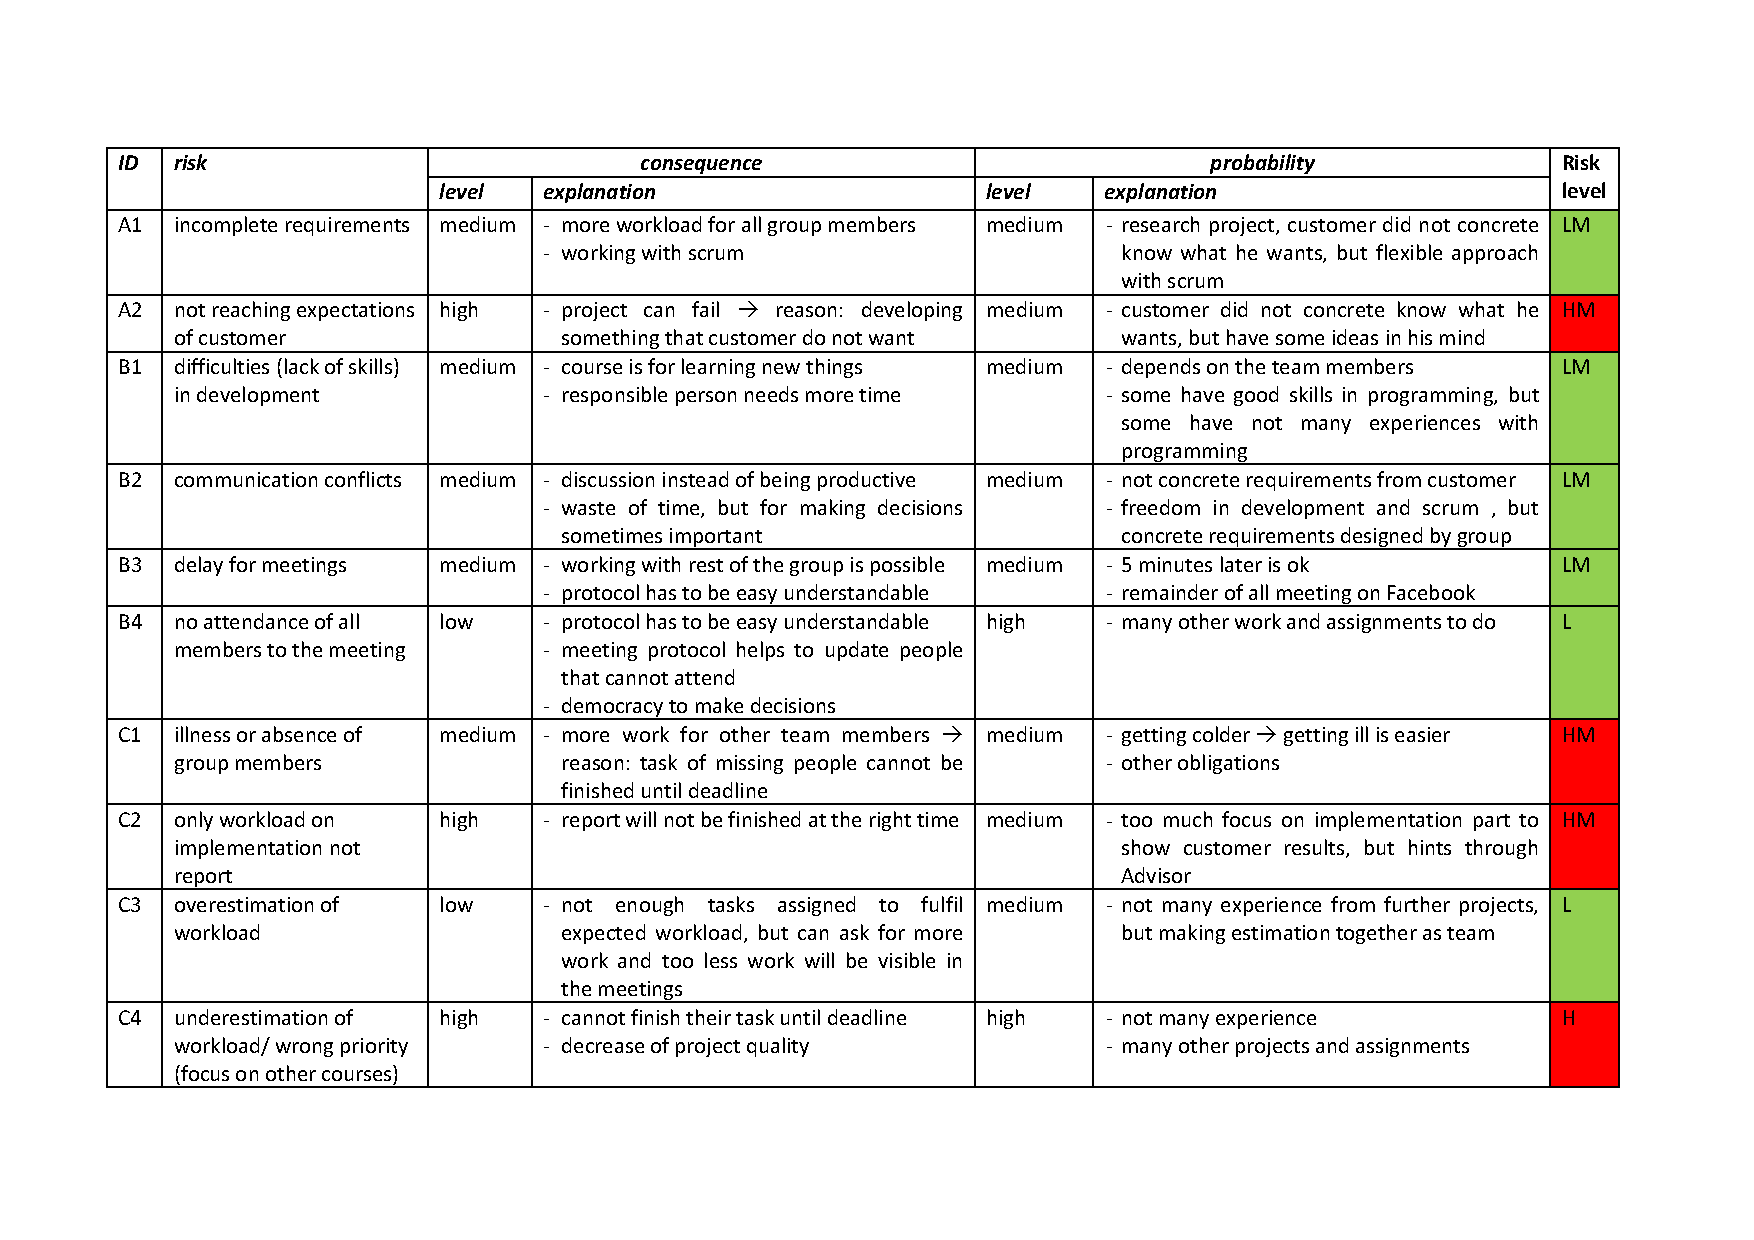
\includegraphics[width=\linewidth]{./Introduction/img/Risk.pdf}
    \caption{Risks for the Alternative Spaces project.}
    \label{fig:IntroRiskManRisks}
\end{sidewaysfigure}